\chapter{Eating Disorder detection}
% deteccion trastornos mentales : dataset, modelos y validacion de los modeloos (resultados)
\label{chap:architecture}
\textit{This chapter presents the methodology used in this work. It describes the overall architecture of the project, with the connections between the different components involved on the development of the project.}

\clearpage
\section{Machine Learning approach}
In order to design the solution we have taken into account the different perspectives that the project could take. To do so, we have decided to first experiment with labelled data in order to perform supervised learning and if we do not achieve good results, we would use other unsupervised learning techniques, as their implementation is much less trivial. In this chapter we are going to talk about the data we have used for this project and the results obtained by using them in Machine Learning models.

In addition, processing has been applied to this information, as we needed to optimise the input of the models so that it would take as much data as possible to make the prediction, which we will also talk about here, the procedures carried out with this data.

Furthermore, the data we are going to analyse are non-numerical, so we will adopt models that use such data and not numbers, a factor that we have had to take into account when selecting learning models. We have mainly focused on the traditional Random Forest, Logistic Regression and SVM models and other more complex pre-trained models such as BERT, specifically using BERT, Mental roBERTa and mBERT.


\subsection{Dataset}
\label{sec:dataset}
% https://arxiv.org/abs/1806.05258
% paper del que se saco
In order to train, validate and then classify and predict, we needed data related to the case study. For this purpose, a search for labelled datasets was made, in which several labelled datasets related to mental illnesses have been found. We decided to use the one introduced in~\cite{https://doi.org/10.48550/arxiv.1806.05258} which investigates the creation of high-precision patterns to identify diagnoses of nine mental illnesses and obtains labeled data without having to manually label it.

The dataset was published in conjunction with the paper, which is called SMHD and is a dataset of social media posts from users with different mental health conditions, including schizophrenia, bipolar disorder, depression, anxiety, obsessive-compulsive disorder, eating disorder, post-traumatic disorder, autism and attention-deficit disorder. In this project we have filtered the data related to Eating Disorders in order to focus on the topic of interest.


% estructura de los datos

In order to be able to go deeper into the data to be able to use them correctly, an analysis of the information present in the SMHD dataset taken has been carried out, in order to subsequently adapt the data to ingest them into the Machine Learning model. To do this, the type of data and its content have been determined in order to decide which are useful and which can be discarded. Subsequently, all this information will be processed in order to adapt it to our use case, in which we want to predict whether a person suffers from Eating Disorder or not by what they write. It should also be noted that, being linguistic and the data being in English, the models have been adjusted to that language, although explorations have been made with other models, as we will discuss in the Section~\ref{sec:models}.

This dataset consists of a set of Reddit posts, concretely 76203 entries of 331 users, labeled with binary classification for suffering an Eating Disorder. The binary label mean of the dataset is 0.345065, that means that around 34.5\% of the post are classified as positive and has an average of 161.13 words per posts, being the maximum a post of 12388 words. This is an strange case because the standard deviation is of 282.8 which indicates that posts are closer to the average number and the maximum number of words of the biggest post is an anomaly. In the Figure~\ref{fig:SMHDwordcloud} the most common used words are displayed.

\begin{figure}[!htp]
    \centering
    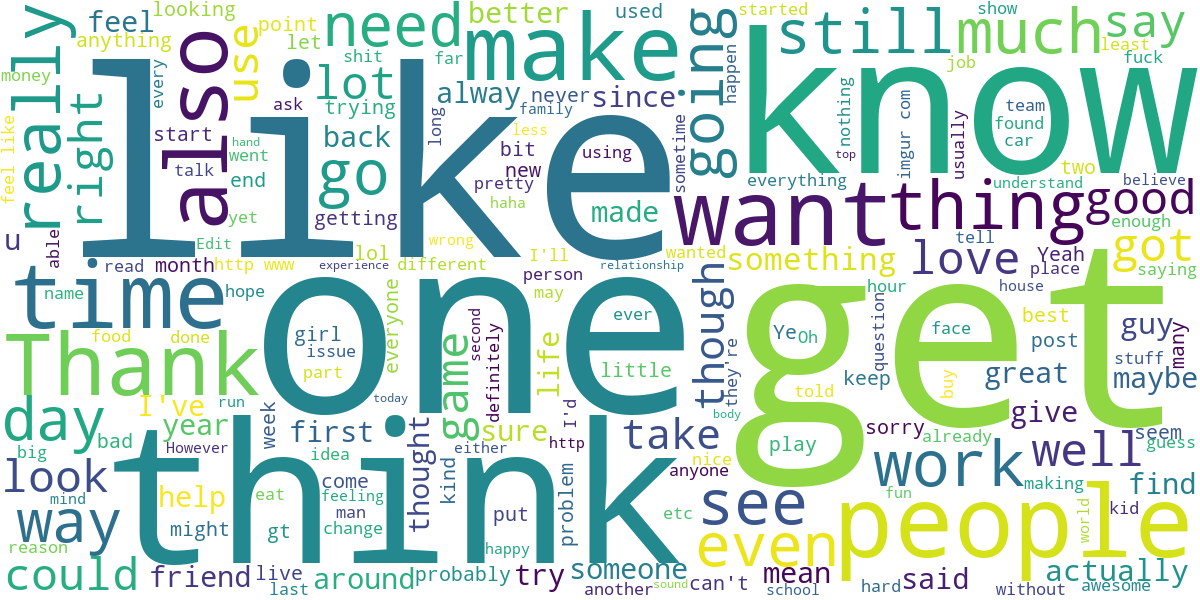
\includegraphics[scale=0.35]{img/detection/SMHD_wordcloud.png}
    \caption{Wordcloud of most common words in SMHD}
    \label{fig:SMHDwordcloud}
\end{figure}


% AQUI O EN CASE STUDY?
\subsection{Twitter Data}
As mentioned above, the aim of this project was to classify posts on social networks, in which we are going to focus mainly on Twitter. To do this, the data used will be tweets from the profile of the person to be analysed, which will then be passed through the Machine Learning algorithm to make the prediction, which is already trained and adapted to the data with the previously mentioned SMHD dataset.

% Scrapping de tweets
To do this, we need to get access to a Twitter API which takes information from the social network via a query. For this, we have used the tool snscrape~\cite{JustAnot83:online}, which allows us to take information from the tweets made by the person to be analysed. It is a Python package that can be easily installed using the pip manager, which allows us to take as many tweets as we want from a profile and put them in a text file in JSON format, as it can be seen in the code block described in Appendix~\ref{appendix:JSONsnscrape}.

% procesamiento de los textos
% recogida de mas datos: pic, username

As you can see in that Appendix, we have a lot of information in addition to what we need for our project, so we have to process the data and keep the ones we are really interested in. For this purpose, a processing method has been implemented within the developed server, which we will discuss in Chapter~\ref{chap:architecture}. In that Chapter we will discuss how we will use other data, as there are also other elements that can be useful for serving them in the application for making it more user-friendly. We are going take this parameters into account for elaborating the API response from our server.

\section{Preprocessing}
Once we had obtained the dataset with which we were going to do the training, we connected to a development environment in order to carry out the pre-processing. We have used the platform of the Jupiter Notebooks department and the Google Collab platform, both of which allow us to create notebooks in which to execute code, specifically Python code, and to have a virtual environment in which to do so.

We load the dataset using Pandas library in the development platform, which allows us to study in depth the characteristics of these as indicated in the Section~ref{sec:dataset} for the information of the SMHD dataset. We can extract different metrics from it, but what we are most interested in is to process the text to put it as input to the model, as it does not work with raw test, but we have to clean it and convert it.

In the Code~\ref{code:preprocessing} we see the treatment given to all the text in the dataset, in which we can see several processes that we are going to explain below.

\begin{lstlisting}[language=Python, caption={Preprocessing used function}, label={code:preprocessing}]
def preprocess(words):
    tokens = nltk.word_tokenize(words)
    porter = nltk.PorterStemmer()
    lemmas = [porter.stem(t) for t in tokens]
    stoplist = stopwords.words("english")
    lemmas_clean = [w for w in tokens if w not in stoplist]
    punctuation = set(string.punctuation)
    words = [w for w in lemmas_clean if  w not in punctuation]
    return words
\end{lstlisting}

\myparagraph{Tokenization}
Tokenization is a process used to change the text and separate the words of a sentence into an array of words separated by a comma, so that the model understands the input we are providing. For serving this purpose, as seen in the code mentioned above, the word\_tokenize method of the NTLK package has been used.

\myparagraph{Stemmization}
Stemmization is a technique whose aim is to reduce a word to its root or base unit, not necessarily a dictionary-based morphological root, but a part equal to or smaller than the word itself. These are typically rule-based algorithms, which can be seen as a heuristic process that cuts off the end of words. In this, a word is taken through a series of conditionals that determine how to cut it.

An example of this might be English suffixes such as "-ed" or "-ing" which do not have much linguistic relevance, being able to relate the words "play", "playing" and "played" which have the same root which is "play."

The stemming algorithm used in this case is Porter's, which is an algorithm from the 1980s whose aim is to erase the common endings of words so that they can be reduced to a common form. It is not very complex and its development is frozen. It is a good algorithm to start introducing in research branches, as it ensures reproducibility, but it is not recommended for use in a complex application due to its limitations.

\myparagraph{Punctuation and stopwords cleaning}
In order to clean the text, we need to eliminate the part of it that doesn't have any linguistic value like punctuation marks(\textit{e.g.} '.','!','?', etc) or stopwords (words, in general adverbs, prepositions, conjunctions and articles, that are meaningless \textit{e.g.} "the", "a", "an", etc.) among others, so we increase the relevance of the remaining items. In order to do so, we take the stopwords provided with the NTLK package and we search for occurences in our text for removing them afterwards.\\


After applying these techniques, we can proceed to pass the data and train the models to fit our data. In the following Section, we will discuss this topic.

\section{Used models}
As explained in the previous Section~\ref{sec:studies}, both traditional and newer machine learning methods have been employed. In this section we will look at what they consist of, the techniques used and the statistical results obtained.

In addition, in each model we will analyse the results obtained with them in order to evaluate the optimisation that they may have. To do this, it is necessary to know some statistical measurements that are going to be explained here but before that, we need to understand the basic concepts for making these statistics, which are the possible results from a prediction.
\begin{itemize}
    \item\textbf{ True positive (TP).} True positive is a result that has been predicted as positive and it is correctly predicted.
    \item\textbf{ False positive (FP).} False positive is a result that has been predicted as positive but it is incorrect, it should have been negative. 
    \item \textbf{True negative (TN).} True negative is a result that has been predicted as negative and it is correctly predicted. 
    \item \textbf{False negative (FN).} False negative is a result that has been predicted as negative but it is incorrect, it should have been positive.
\end{itemize}

With these concepts explained, we can dig into the concepts introduced before that we will use for evaluation of the models which are precision, recall, accuracy or F1-score.

\begin{itemize}
    \item \textbf{Precision.} Precision is defined as the number of true positives that have been among all the positive predictions. In an equation it would look like the following.
    \begin{equation}
        precision = \frac{TP}{TP + FP} 
    \end{equation}
    \item \textbf{Recall.} Recall is the measurement of the capacity of the model for classifying true positives.
    \begin{equation}
        recall = \frac{TP}{TP + FN} 
    \end{equation}
    \item \textbf{Accuracy.} Accuracy is the measure of the correct predictions that have been made.
    \begin{equation}
        accuracy = \frac{TP + TN}{TP + FP + TN + FN} 
    \end{equation}
    \item \textbf{F1-score.} F1-score is the mean of precision and recall
    \begin{equation}
        F1-score = \frac{2 * precision * recall}{precision + recall} 
    \end{equation}
    
\end{itemize}

\label{sec:models}
\subsection{Traditional Models}
In this project, we call traditional models those models that have not been pre-trained and are historically more consolidated in the field of Machine Learning and Artificial Intelligence, despite this being a relatively new and booming field.

\subsubsection{Random Forest}
Random Forest is a decision tree-based Machine Learning algorithm used for classification or regression of data by constructing many decision trees when training the model. In the case of classification, the output tree is the class selected by the largest number of trees, as in our case. A representation of it can be seen in the Figure~\ref{fig:random-forest}.

\begin{figure}[!htp]
    \centering
    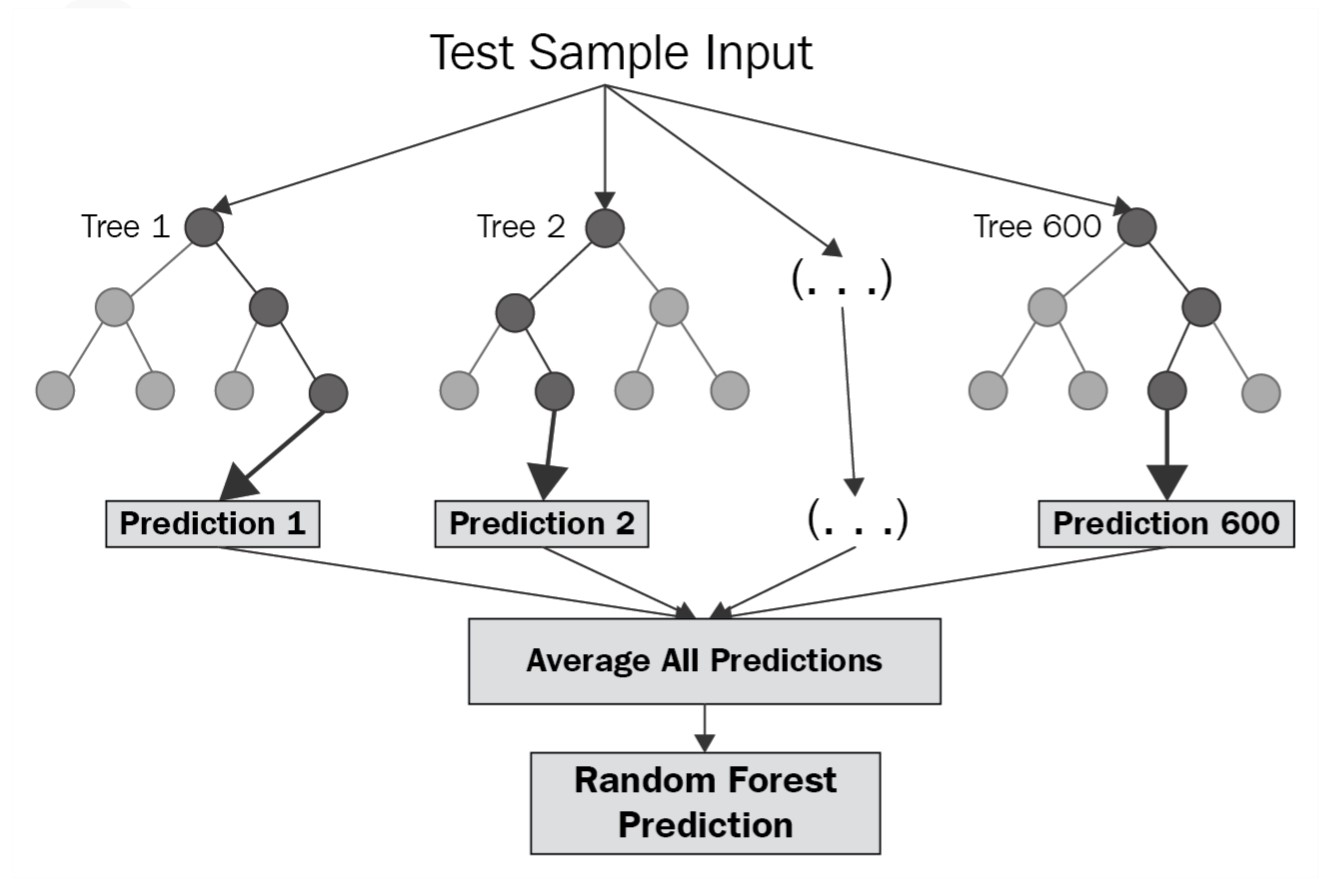
\includegraphics[scale=0.3]{img/detection/random-forest.jpg}
    \caption{Random Forest model representation}
    \label{fig:random-forest}
\end{figure}

This algorithm corrects the flaw in decision trees of overfitting the training set, i.e. overtraining a learning algorithm so much that it is only effective under very specific conditions, those of the training data.

%% HABLAR DE HIPERPARAMETROS
In our case, we have used the Random Forest algorithm of the sklearn package with a number of estimators equal to 400, as well as tuning other parameters of the model, as they have been optimised by using GridSearchCV, a tool packaged with the sklearn library that allows us to optimise hyperparameters of the model.


\begin{table}[!htp]
\centering
\begin{tabular}{|l|l|l|l|}
\hline
         & precision & recall & f1-score \\ \hline
0        & 0.81      & 0.91   & 0.86     \\ \hline
1        & 0.91      & 0.81   & 0.86     \\ \hline
accuracy & 0.86      & 100    &          \\ \hline
\end{tabular}
\caption{Statistics for Random Forest}
\label{tab:RandomForestStatistics}
\end{table}

\subsubsection{SVM}
The Support Vector Machine algorithm, also known as SVM, is used in classification and regression problems, but in our case we will focus on the former. The objective of this is to find a hyperplane that best separates two different classes of data points,\textit{ i.e.} with the widest margin between the two classes. 

This margin is defined as the maximum width of the region parallel to this hyperplane that has no interior data points. This algorithm only works on problems that allow linear separation, maximising the aforementioned margin as it can be seen in Figure~\ref{fig:SVM}.

\begin{figure}[!htp]
    \centering
    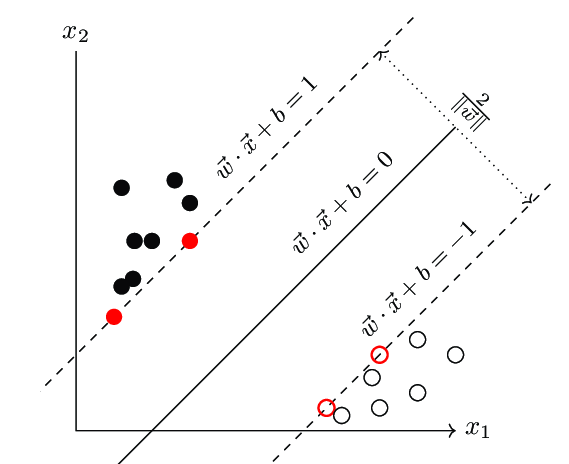
\includegraphics[scale=0.4]{img/detection/SVM.png}
    \caption{SVM model representation}
    \label{fig:SVM}
\end{figure}

%% HABLAR HIPERPARAMETROS
In our case, the configurable hyperparameters of the model have been evaluated by means of a GridSearchCV, in order to optimise it as much as possible to our data. With this, the statistics shown in table \ref{tab:SVM-statistics} have been obtained.

\begin{table}[!htp]
\centering
\begin{tabular}{|l|l|l|l|}
\hline
         & precision & recall & f1-score \\ \hline
0        & 0.78      & 0.89   & 0.83     \\ \hline
1        & 0.89      & 0.77   & 0.83     \\ \hline
accuracy & 0.83      & 100    &          \\ \hline
\end{tabular}
\caption{Statistics for SVM model}
\label{tab:SVM-statistics}
\end{table}

\subsubsection{Logistic Regression}
This model is within supervised learning and is used to predict the categorical dependent variable given a set of independent variables. This predicted output can take both categorical and discrete values and is used for classification problems. In this regression, an attempt is made to fit the values within an "S" shaped logistic function that predicts between two maximum values, either 0 or 1 as can be seen in Figure~\ref{fig:LogisticRegression}.

\begin{figure}[!htp]
    \centering
    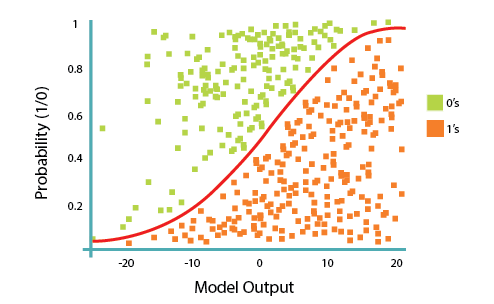
\includegraphics[scale=0.6]{img/detection/LogisticRegression.png}
    \caption{Logistic Regression representation model}
    \label{fig:LogisticRegression}
\end{figure}

Again, we proceeded to see which were the best hyperparameters for this model by using GridSearchCV, obtaining the results shown in Table~\ref{tab:LogisticRegressionStatistics}.



\begin{table}[!htp]
\centering
\begin{tabular}{|l|l|l|l|}
\hline
         & precision & recall & f1-score \\ \hline
0        & 0.80      & 0.91   & 0.85     \\ \hline
1        & 0.91      & 0.79   & 0.85     \\ \hline
accuracy & 0.85      & 100    &          \\ \hline
\end{tabular}
\caption{Statistics for Logistic Regression model}
\label{tab:LogisticRegressionStatistics}
\end{table}

\subsection{BERT Models}
After explaining the traditional models as we have called them in the present project, in which we had a mathematical algorithm that had to be trained to optimise the models to subsequently make the predictions, we are going to explain the BERT models (Bidirectional Encoder Representations from Transformers). 

BERT models are pre-trained and open source machine learning techniques based on neural networks for NLP developed by Google in 2018. These algorithms have been used in the company's search engine since 2019. BERT makes use of Transformer, an attention mechanism that learns the contextual relationships between words and includes two different mechanisms, an encoder that reads the input text and a decoder that produces a prediction. This encoder is the necessary element, because BERT's goal is to generate a language model.

BERT models can be used for a number of different linguistic tasks by adding only a small layer to the core model. In classification tasks, as is the case in this project and in sentiment analysis, they are performed in a similar way to Next Sentence Prediction (NSP), by adding a classification layer on top of the output of the token transformer (CLS).

In the NSP training process, the model is provided with pairs of sentences as input and learns whether the second sentence of the pair is the next sentence in the original document to learn about the context. 50\% of the input sentence pairs are the subsequent sentences in the original document and the other 50\% are randomly chosen and disconnected sentences. In order to process the input text the following steps are needed to be performed, as it can be seen in Figure~\ref{fig:BERTinput}.

\begin{enumerate}
    \item A CLS token and a SEP token are inserted at the beginning and end of each sentence respectively.
    \item A phrase embedding indicating phrase A or phrase B is added to each token.
    \item A positional inlay is added to each token to indicate its position in the sequence.
\end{enumerate}

\begin{figure}[!htp]
    \centering
    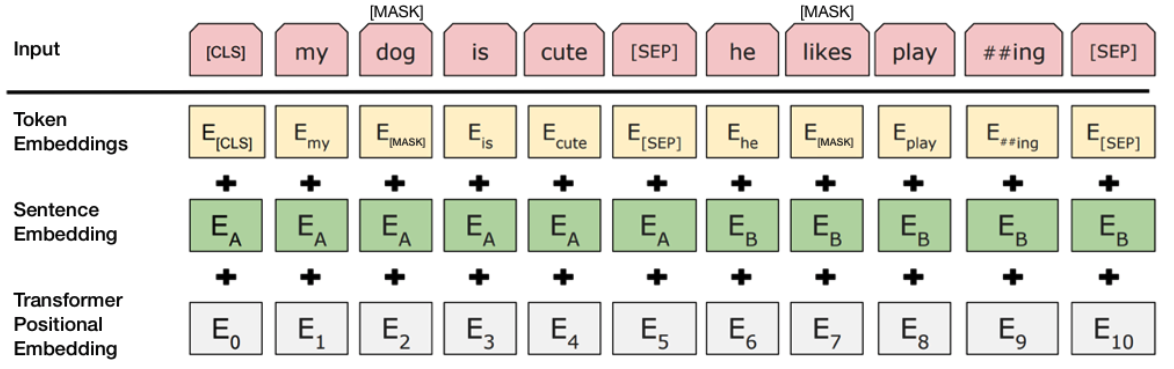
\includegraphics[scale=0.35]{img/detection/BERTinput.png}
    \caption{BERT input processing in NSP}
    \label{fig:BERTinput}
\end{figure}
Once the input text has been pre-processed, to make the prediction of the second sentence over the first, the following is needed.

\begin{enumerate}
    \item Introducing the sequence to the Transformer model.
    \item The output of the [CLS] token is transformed into a 2x1 vector using one of classification.
    \item Calculate the probability with softmax or normalised exponential function.
\end{enumerate}

BERT models, as they are pre-trained and open source, they can be packed with certain contextual representations because the model can be pretrained with different inputs. In our case, we have experimented with pure BERT implementation and two variants which are Mental roBERTa and mBERT using the Google Collab platform. We are going to discuss the results of those analysis here.

\myparagraph{BERT}
We implemented the BERT model without any specialization in its pre-training, using the bert-based-cased tokenizer and the BERTClassifier model from the Transformers library, and obtained the results shown in Table~\ref{tab:BERTstatistics}.

\begin{table}[!htp]
\centering
\begin{tabular}{|l|l|l|l|}
\hline
precision & recall & f1-score  & accuracy \\ \hline
0.566      & 0.529   & 0.495      &  0.529 \\ \hline
\end{tabular}
\caption{Statistics for BERT model}
\label{tab:BERTstatistics}
\end{table}
The results were not as good as expected so we decided to improve them by using other BERT variants pretrained with specific data that is closer to our case study.

\myparagraph{Mental roBERTa}
This model is pretrained with post related to mental health problems, which we though it would introduce an improvement in our statistics and the results we obtained were as in Table~\ref{tab:MentalroBERTastatistics}.
\begin{table}[!htp]
\centering
\begin{tabular}{|l|l|l|l|}
\hline
precision & recall & f1-score  & accuracy \\ \hline
0.737      & 0.735   &  0.735      &  0.735 \\ \hline
\end{tabular}
\caption{Statistics for Mental roBERTa model}
\label{tab:MentalroBERTastatistics}
\end{table}

As expected, results were much better using Mental roBERTa but still distant from what we achived with the other models.
\myparagraph{mBERT}
mBERT model is a regular implementation for BERT pretrained with data from more than a 100 languages, so it can provide support for multilingual applications. As it is now, our model only supports text in English but we would like to extend this functionality in the future and this is why we made test with this specific model. The obtained results are as discussed in Table~\ref{tab:mBERTstatistics}.
\begin{table}[!htp]
\centering
\begin{tabular}{|l|l|l|l|}
\hline
precision & recall & f1-score  & accuracy \\ \hline
0.651      & 0.647   & 0.647      &  0.647 \\ \hline
\end{tabular}
\caption{Statistics for mBERT model}
\label{tab:mBERTstatistics}
\end{table}

And again, as expected the model works much worse than Mental roBERTa as it is not specialized in Mental Health problems but on the other hand, we could win multilanguage support with it. \\

There are more variants that could be implemented such as patentBERT(fine-tuned to perform patent classification), bioBERT (for biomedical text mining) or SciBERT (for scientific texts), but as the results with BERT were not as good as we obtained with the traditional models, we decided to stop working but it is a field from this project that could be investigated for optimising in the future.



\subsection{Decision}
% exponer las medidas tomadas para cada modelo y dar una valoracion
As we have been reviewing, we have analysed the performance of the models Random Forest, SVM, Linear Regression and BERT (with two additional variants pretrained with specific data) and we have now the necessary criteria to make a decision on what model to choose.

So far, the model that throws the best results is \textbf{Random Forest}, which has also a small execution time, so we have decided that it will be our main model in our project. We could include mBERT as well for languages that are not English so we will review its viability as well, keeping as principal algorithm the Random Forest.
